%!TEX root = ./exercice2.tex

\section{Parametric Identification of an Active Suspension System}
In this section we identify a model between the current reference for the DC motor and the acceleration of the sprung mass of the active suspension system in Figure~\ref{fig:active_suspension}. 
Therefore, we use the time-domain data CE2.mat. This file contains the input $u$ and the output signal $y$ of the system with a set of $N = 2044$ data and a sampling time of $T_e = 0.03$. 
\begin{figure}[h]
	\centering
	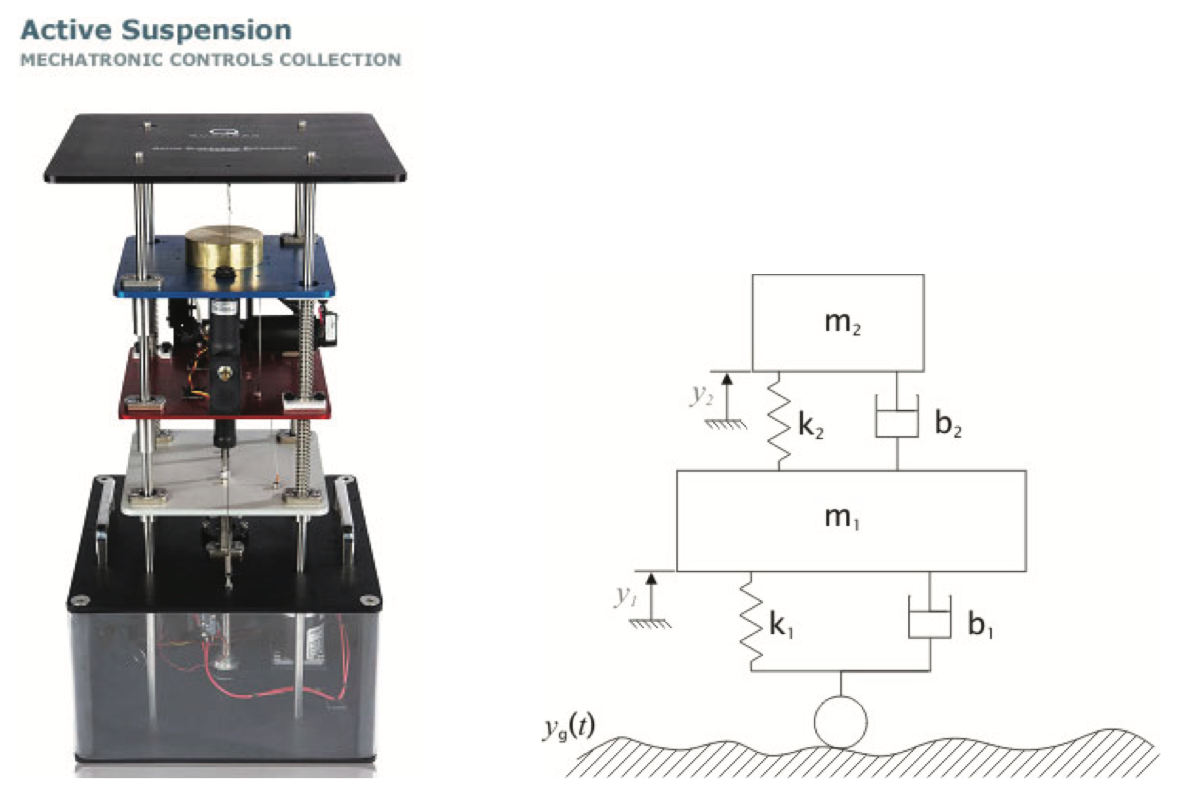
\includegraphics[height=5.5cm]{figures/active_suspension.png}
	\caption{Output of the system}\label{fig:active_suspension}
\end{figure}
Before we start with the identification procedure, we remove the mean value of the input and output with the MATLAB \texttt{detrend} command and generate a data object with the MATLAB \texttt{iddata}.

\subsection{Order Estimation}
It is one of the goals of system identification to find the simplest model, which meets the desired criteria. Therefore, the model order estimation plays an important role in the procedure. In this section, we will focus on finding the order for the Active Suspension System. 

In the first approach, we will use the ARX structure. As the loss function $ J(\hat{\theta}) /N $ for this structure is monotonically non-increasing with respect to the number of the parameter estimates (dimension of $\theta$), the model order can be estimated by analyzing the shape of the loss function. We set the delay to $n_k = 0$, the order of the nominator of the plant model $n_b$ equal to the order of the denominator $n_a$ and choose a maximum order of $n=10$. In doing so, we obtain $10$ different ARX models. The corresponding loss function can be seen in Figure~\ref{fig:loss_fcn}. 

\begin{figure}[h]
	\centering
	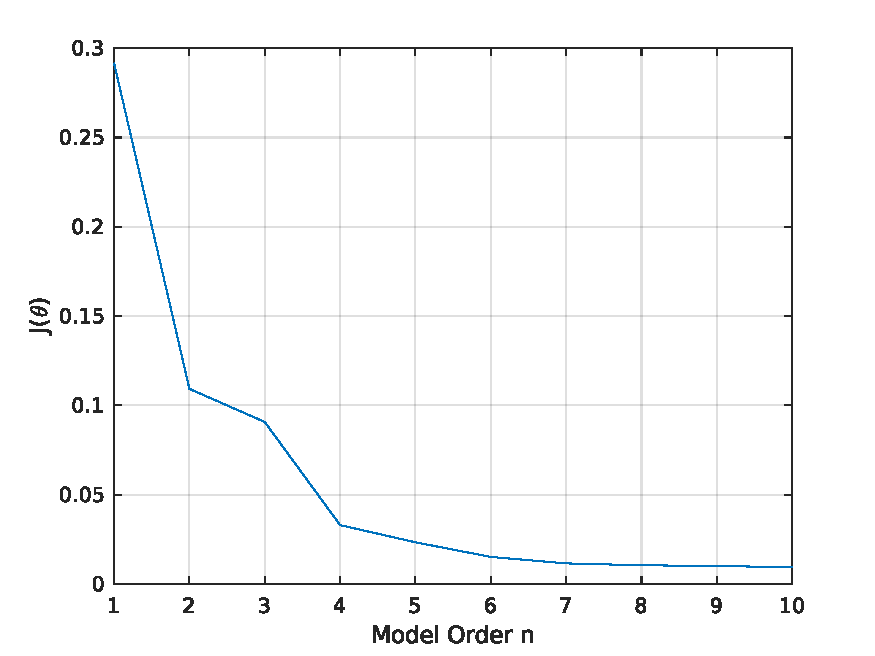
\includegraphics[height=6cm]{figures/Loss_fcn.pdf}
	\caption{Output of the system}\label{fig:loss_fcn}
\end{figure}

As the slope of the loss function is close to zero for $n \geq 6 $ we choose a model order equal to $n = 6.$ \\

Afterwards we want to validate the chosen order by using the zero/pole cancellation method applied to the ARMAX structure for different models. 
We set the order of the plant model $n_a$ and $n_b$ and the order of the noise model $n_c$ to the same value, that means $n_a = n_b = n_c = n $ and the delay equal to one, $n_k = 1$. 
As the estimated order is $6$ according to the loss function method, we choose $ n_{min} \leq n \leq n_{max}$ with $ n_{min} = 5$ and $n_{max}=8$. With the MATLAB command \texttt{iopzplot} we plot the zero/pole map of this $4$ different models, which can be seen in Figure~\ref{fig:zero_pole}. 
As we use noisy data for our identification, an exact zero pole cancellation is impossible (that means an exact overlap between a zero 'o' and a cross 'x' in the map respectively). To solve this issue, a confidence interval with a size of two times their standard deviation $\pm 2 \sigma$ for each pole and zero is plotted. At that point, one zero/pole cancellation indicates, that the order of the model is overestimated by one. 

\begin{figure}[h]
	\centering
	\begin{subfigure}{.49\textwidth}
		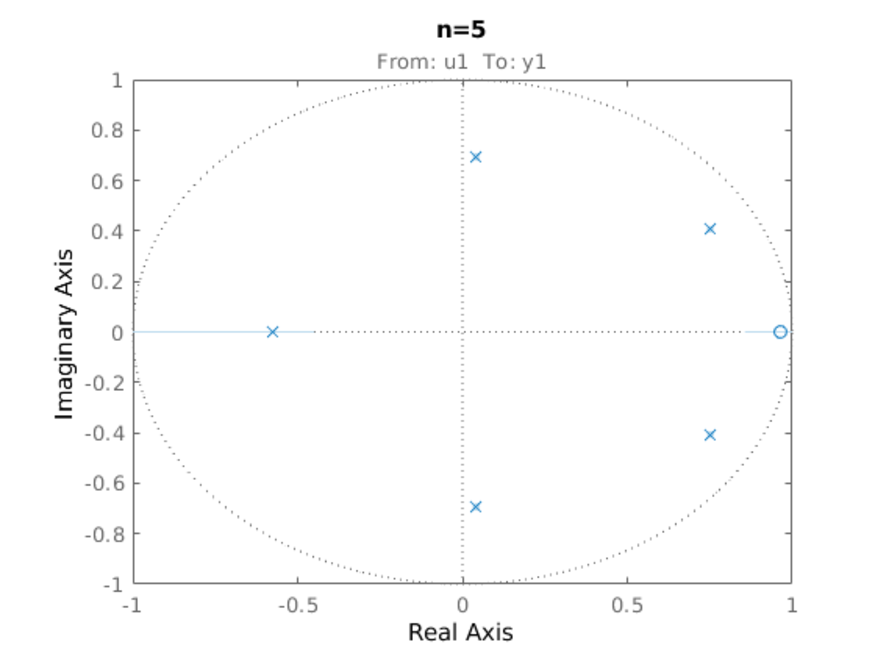
\includegraphics[height=6.5cm]{figures/zp5.pdf}
		\subcaption{Zero/pole map for $n_a = n_b = n_c = 5 $}\label{fig:zp5}
	\end{subfigure}\hfill
	\begin{subfigure}{.49\textwidth}
		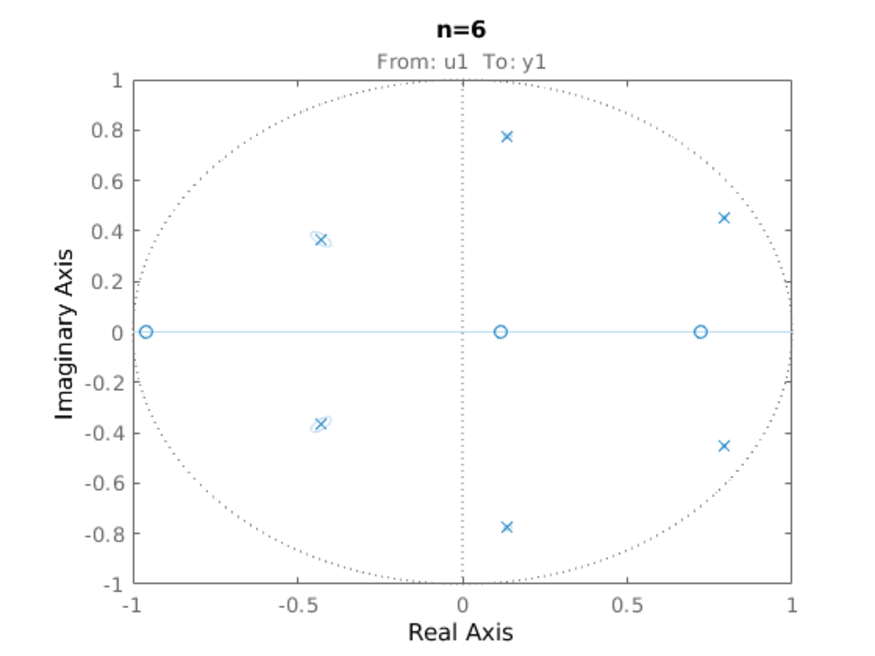
\includegraphics[height=6.5cm]{figures/zp6.pdf}
		\subcaption{Zero/pole map for $n_a = n_b = n_c = 6 $}\label{fig:zp6}
	\end{subfigure}
	\begin{subfigure}{.49\textwidth}
		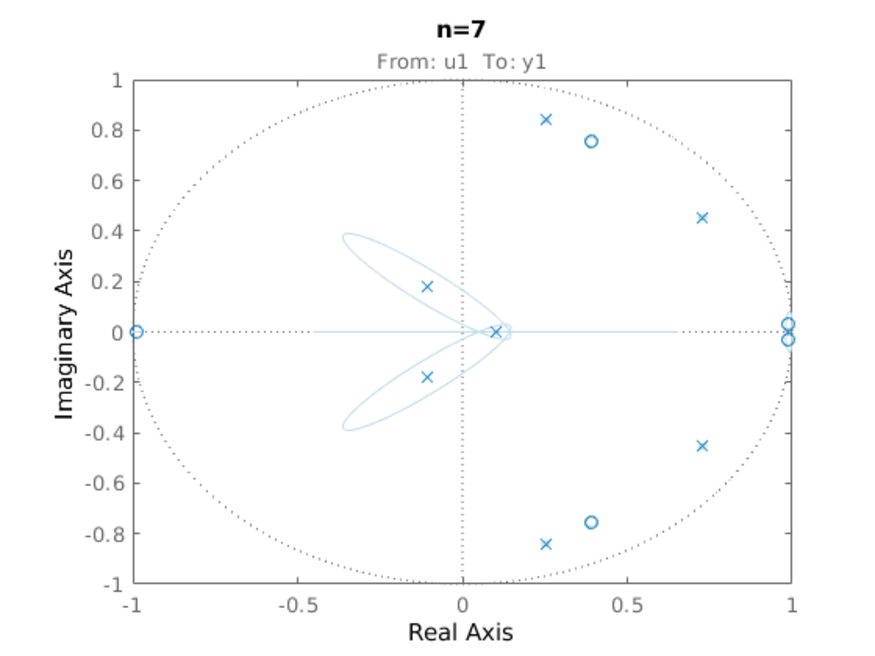
\includegraphics[height=6.5cm]{figures/zp7.pdf}
		\subcaption{Zero/pole map for $n_a = n_b = n_c = 7 $}\label{fig:zp7}
	\end{subfigure}\hfill
	\begin{subfigure}{.49\textwidth}
		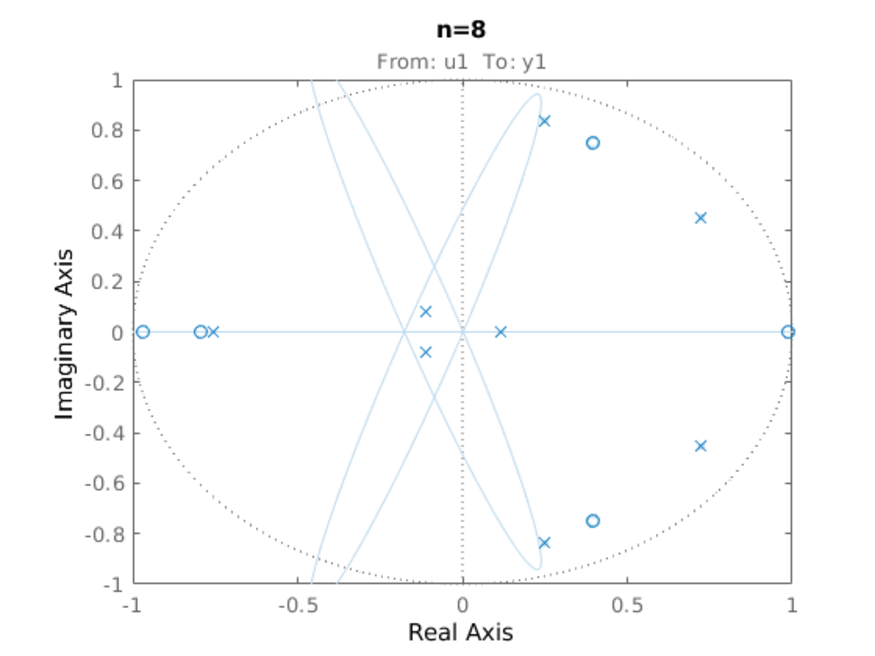
\includegraphics[height=6.5cm]{figures/zp8.pdf}
		\subcaption{Zero/pole map for $n_a = n_b = n_c = 8 $}\label{fig:zp8}
	\end{subfigure}
	\caption{Zero/pole map for different ARMAX models}
	\label{fig:zero_pole}
\end{figure}

The zero/pole cancellation method validates our chosen order $n=6$. For an order of $n=7$ the confidence intervals are significantly larger than for lower orders. That is why we cannot determine the exact value of the poles. \textcolor{red}{Begründung} \\

As a next step, the delay $n_k$ is estimated. This is done by inspecting the impulse response of the system. As the impulse response is equal to the parameters $b_k$ of a FIR model, we use a high order FIR model to plot it. All we have to consider is that the number of parameters $m$ of this model is bigger then the settling time of the impulse response $g(t)$. As $g(t)$ is approximately zero after $ 1 s$ we set the model order to $m = 40$ due to the sampling time $T_e = 0.03 s$.
The time delay $d$ of the system can then be obtained as the number of the first values of the impulse response, that is the first parameters of the FIR model, that are equal to zero. 
However, using noisy data none of the values will be equal to zero. In this case a value can be considered as zero is $ 0 \in \left[b_k -2 \sigma_k, b_k + 2\sigma_k \right] $ with $\sigma_k$ as the standard deviation of the k-th component. 

In MATLAB, we create the FIR model with the command \texttt{oe}. The code can be seen in Listing~\ref{lst:delay}


Figure~\ref{fig:fir40} shows the impulse response and Figure~\ref{fig:fir40_dev} the parameters with their corresponding confidence interval. As the second value of the impulse response is approximately zero, we estimate the delay as $d=1$ and obtain $n_k = d + 1 = 2$. 

\begin{figure}[h]
	\centering
	\begin{subfigure}{.49\textwidth}
		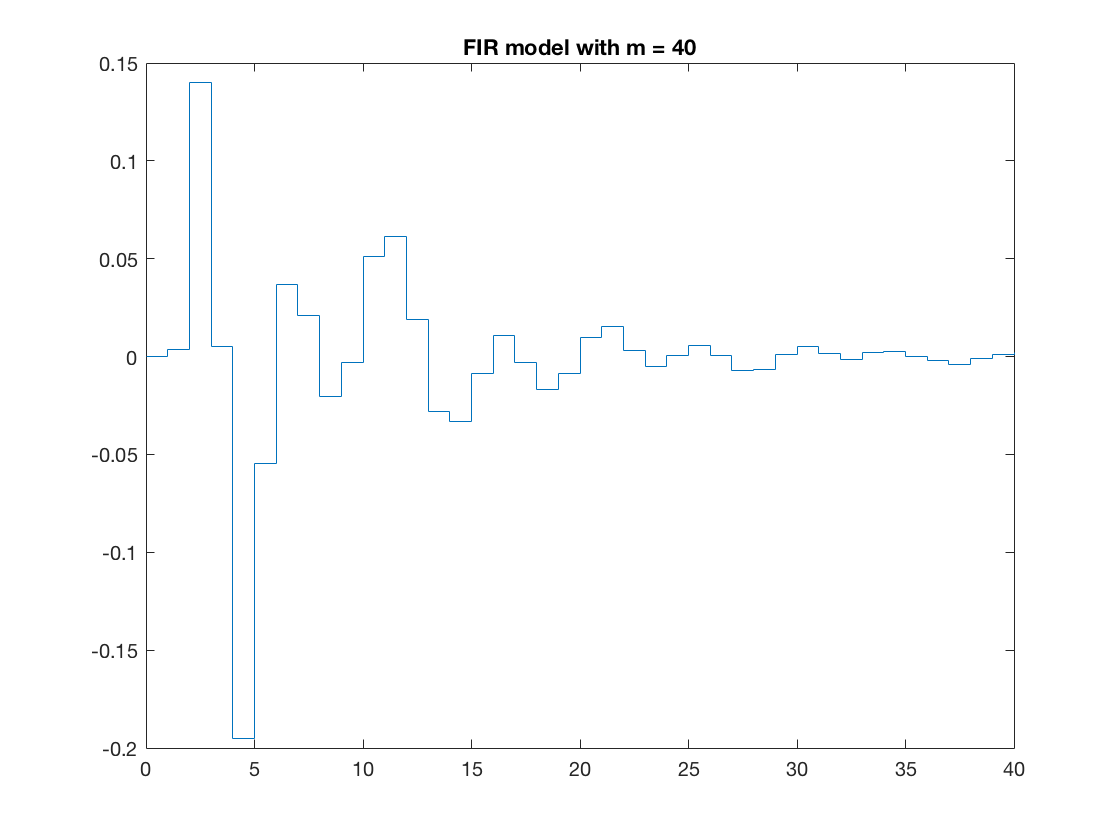
\includegraphics[height=5.5cm]{figures/fir40.png}
		\subcaption{Impulse response of the system with a FIR model. It can be seen, that the second value is nearly equal to $0$, what implies a delay of $1$}\label{fig:fir40}
	\end{subfigure}\hfill
	\begin{subfigure}{.49\textwidth}
		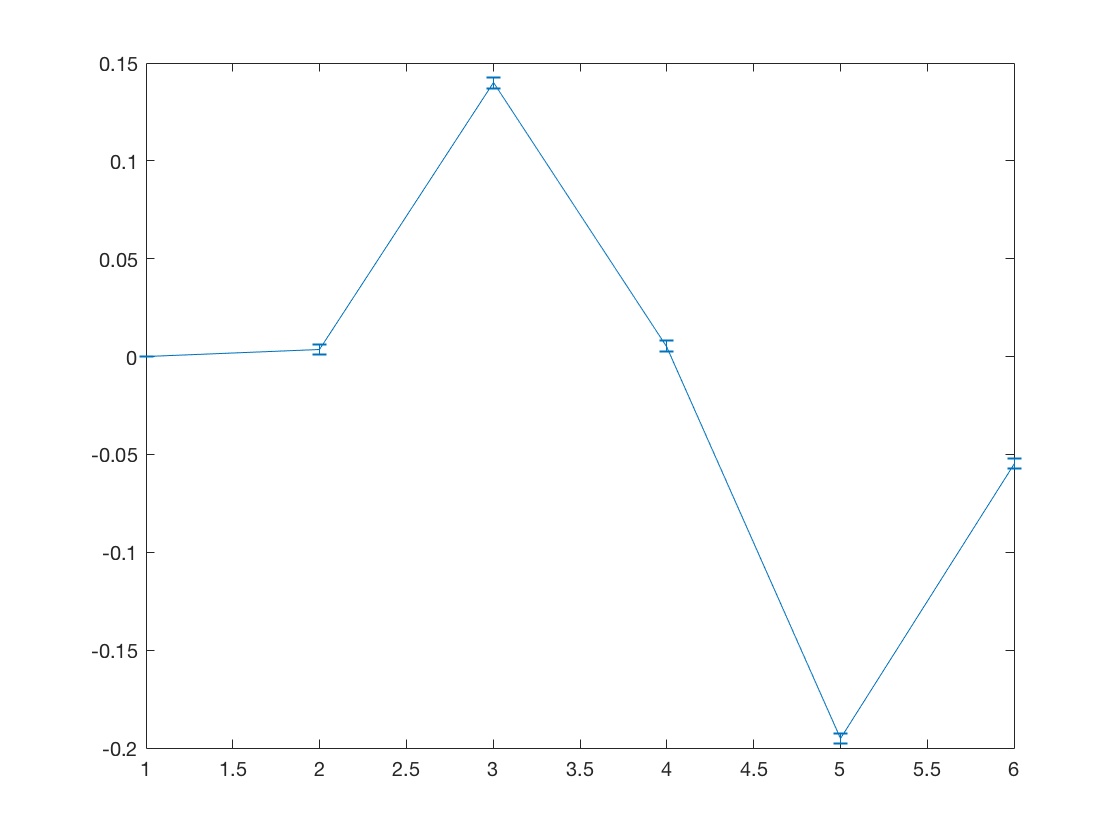
\includegraphics[height=5.5cm]{figures/fir40_dev.png}
		\subcaption{The first six parameters and ther confidence interval}\label{fig:fir40_dev}
	\end{subfigure}
	\caption{Estimation of the delay with a high order FIR model}
	\label{fig:delay}
\end{figure}

As the last step, the number of the parameters in the numerator $n_b$ is estimated. This is done by comparing the loss function of different ARX models with a value of $n_b$ as follows: $1 \leq n_b \leq n  - n_k + 1 = 6 - 2 + 1 = 5$. This is done with the MATLAB variable \texttt{M.EstimationInfo.LossFcn}. The results can be seen in Table~\ref{tab:denom}.

\begin{table}[h]
	\centering
	\begin{tabular}{l|c}
	\hline
	\hline
	\textbf{Number of parameters $n_b$} & \textbf{Loss function of ARX model}\\
	\hline
		$5$ & $0.0153$ \\ \hline
		$4$ & $0.0161$ \\ \hline
		$3$ & $0.0204$ \\ \hline
		$2$ & $0.0529$ \\ \hline
		$1$ & $0.0711$ \\ \hline
	\hline
	\end{tabular}
	\caption{Loss function for different numbers of parameter in the denominator}
	\label{tab:denom}
\end{table}

As there is only a small reduction of the loss function between $n_b = 5$ and $n_b = 4$ compared to the other steps, we decide to choose $n_b = 4$. 

Summarized, our estimated parameter values are $n_k = 2$, $n_a = 6$ and  $n_b = 4$. \\

Finally, we compare our results with those proposed by MATLAB with the commands \texttt{struc}, \texttt{arxstruc} and \texttt{selstruc}. 
With \texttt{struc} we generate $1000$ model-order combinations for the ARX model estimation ($n_a = n_b = n_k = 10)$. Afterwards the loss functions for all the ARX models are calculated with \texttt{arxstruc}. \texttt{selstruc} then allows us to select a model order by showing the values of the different loss functions graphically (Figure~\ref{fig:selstruc}). 

\begin{figure}[h]
	\centering
	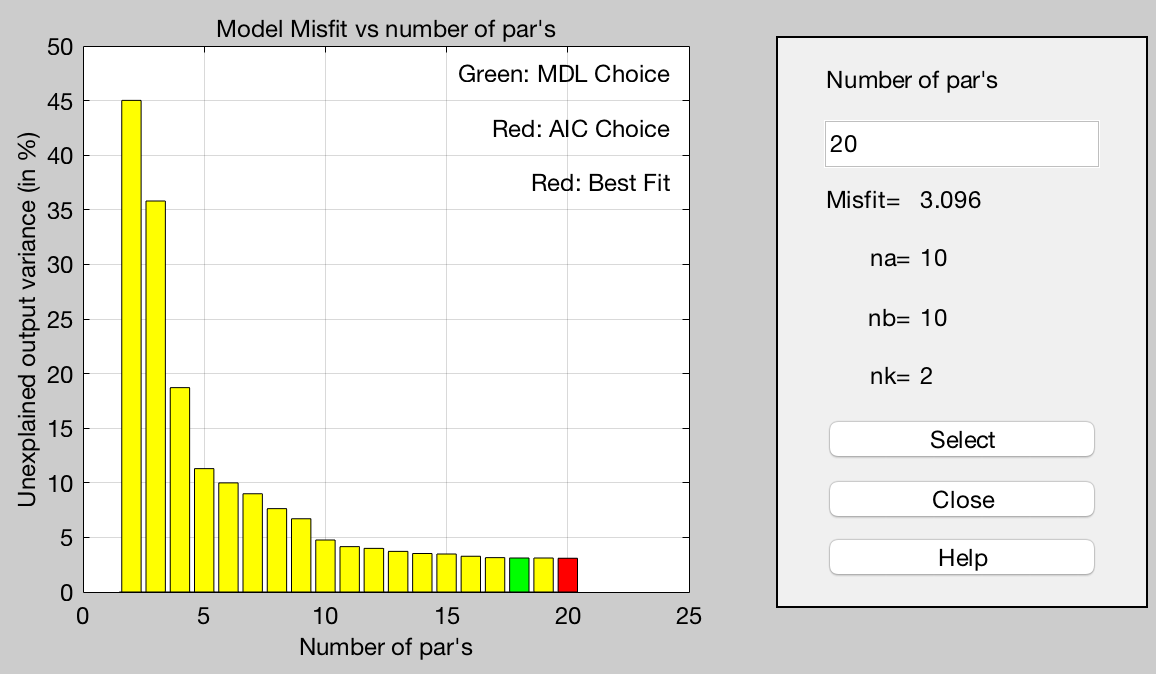
\includegraphics[height=6cm]{figures/selstruc.png}
	\caption{Loss functions calculated with \texttt{arxstruc}}\label{fig:selstruc}
\end{figure}

The order proposed by MATLAB via \texttt{struc}, \texttt{arxstruc} and \texttt{selstruc} is significantly larger ($n = 10$). This is due to the fact, that MATLAB tries to fit the noise as well and not just only the real data. It can be seen in Figure~\ref{fig:selstruc} that the output variance is almost constant for more than $10$ parameters. As we want a good trade-off between computational cost and the variance, $10$ parameters seems to be a reasonable choice. This coincides with the choice we made before, since $n_a + n_b = 6 + 4 = 10$. 

\subsection{Parametric Identification}
In this section, we want to create different parametric models using the estimated values for the parameters $n_a$, $n_b$ and $n_k$ from the previous section. Therefore, we use various MATLAB commands. We create ARX model, an Instrumental variables method model, an ARMAX model, an Output error structure model, a  Box-jenkings model and a State space model.\\
Doing that, we divide the data in to different parts. The first one we use for the model identification and the second one for the model validation. 
The code for this can be seen in Listing~\ref{lst:parametric}.  

\subsection{Model Validation}
As a final step, we want to validate the identified parametric models. Therefore, the data set of $N = 2044$ is again partitioned in two parts. The second half of the data, that has not been used for the identification, is used to validate the models. \\
First, we compare the output of the models with the measured output of the second half of the data.  Thereby, the same input is applied to the model and the system. 

\begin{figure}[h]
	\centering
	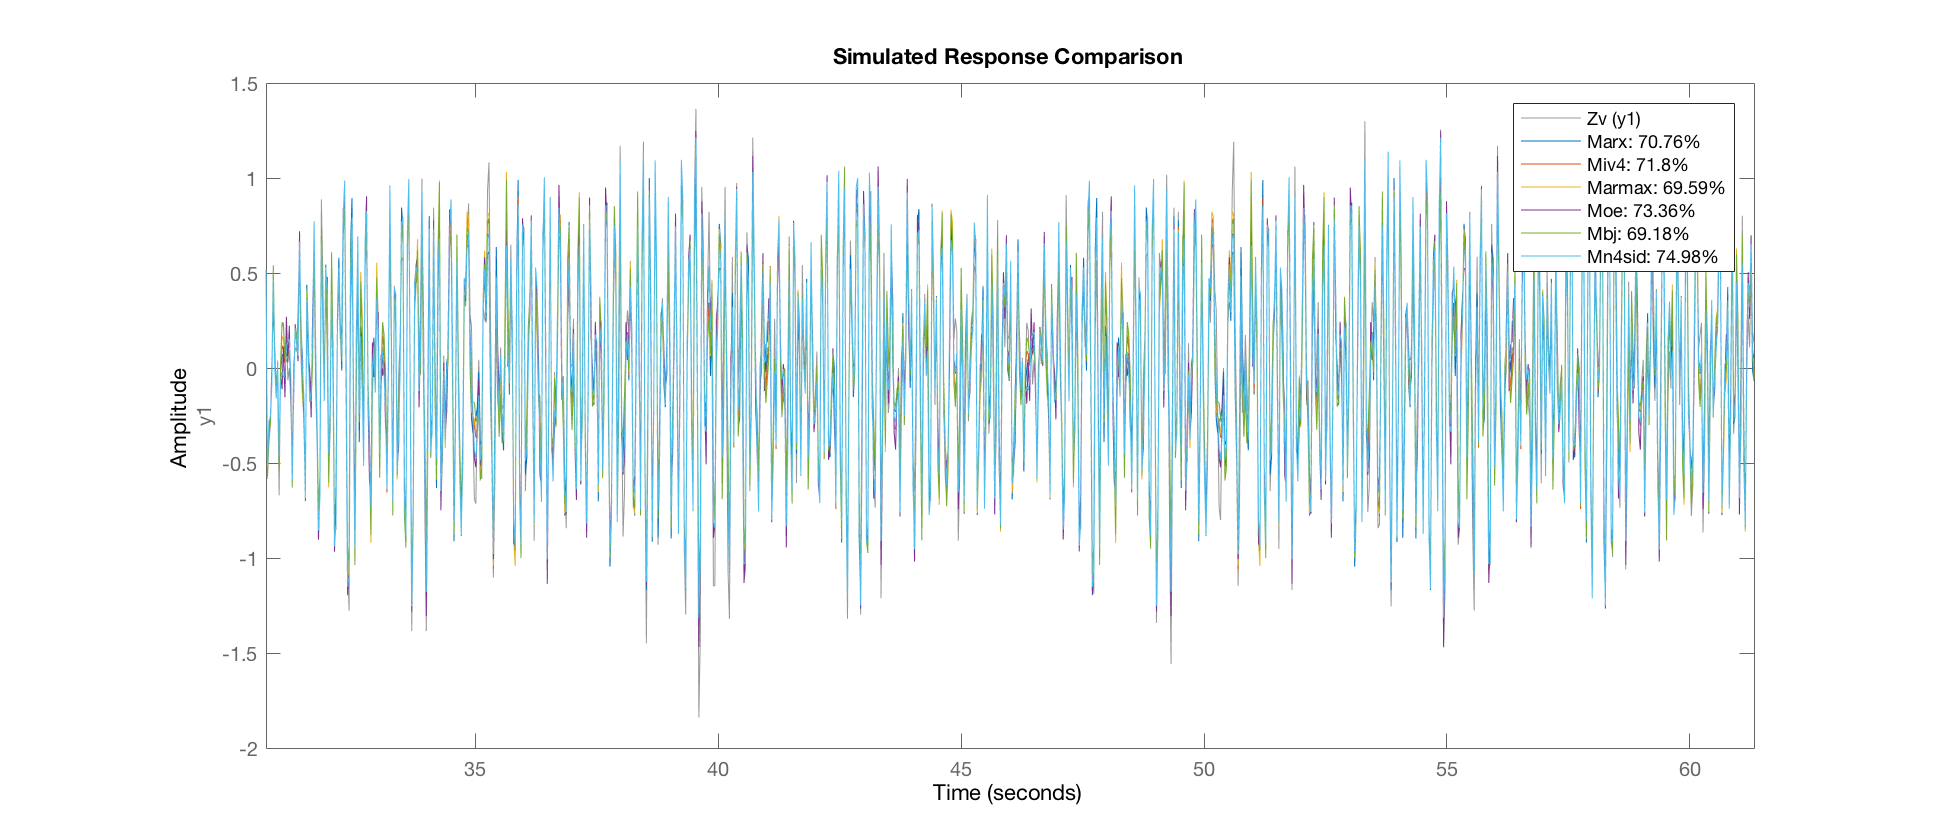
\includegraphics[height=7cm]{figures/comparison.png}
	\caption{Comparison of the measured output with the output of the models with the same input each time. The MATLAB command \texttt{compare} is used. }\label{fig:comparison }
\end{figure}

According to this, the best model is the State Space Model with a fit of $74.98 \% $


\begin{figure}[h]
	\centering
	\begin{subfigure}{.49\textwidth}
		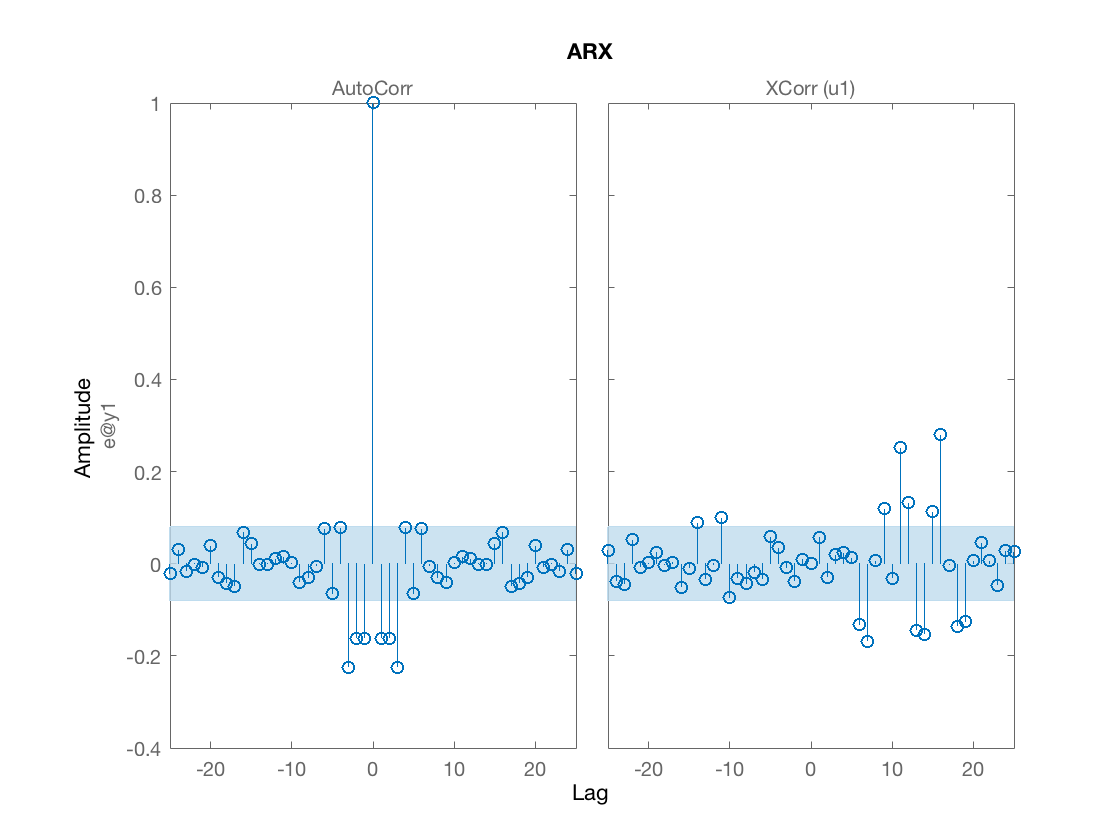
\includegraphics[height=5.5cm]{figures/v_arx.png}
		\subcaption{Whiteness test and cross-correlation test of the ARX model}\label{fig:v_arx}
	\end{subfigure}\hfill
	\begin{subfigure}{.49\textwidth}
		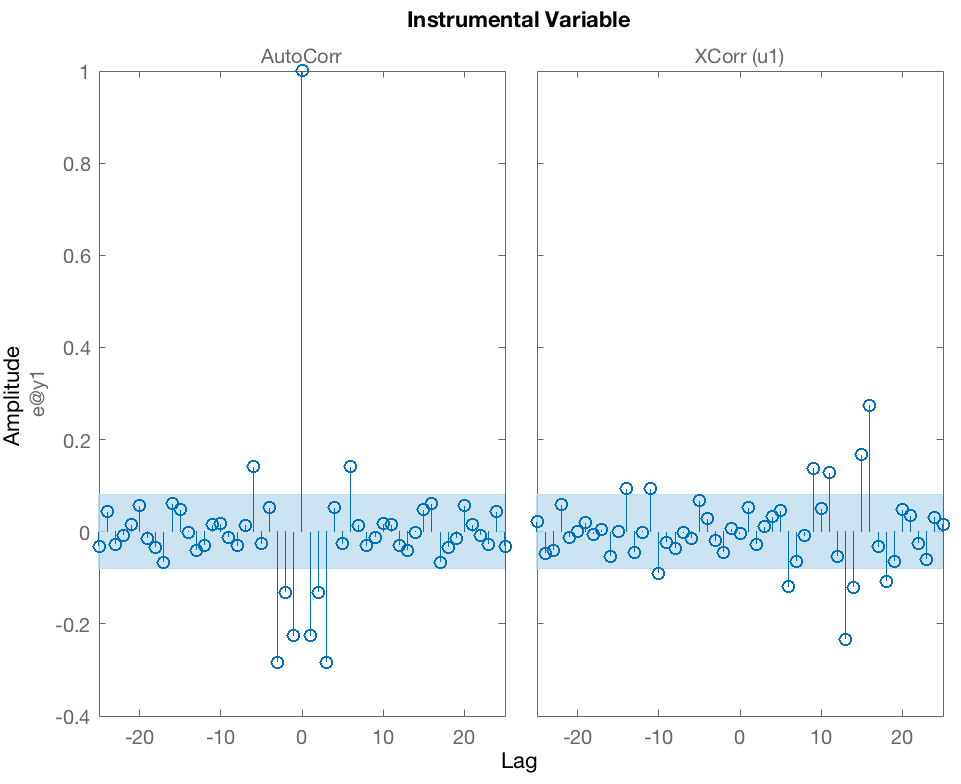
\includegraphics[height=5.5cm]{figures/v_iv.png}
		\subcaption{Whiteness test and cross-correlation test of the Instrumental Variables method}\label{fig:v_iv4}
	\end{subfigure}
	\begin{subfigure}{.49\textwidth}
		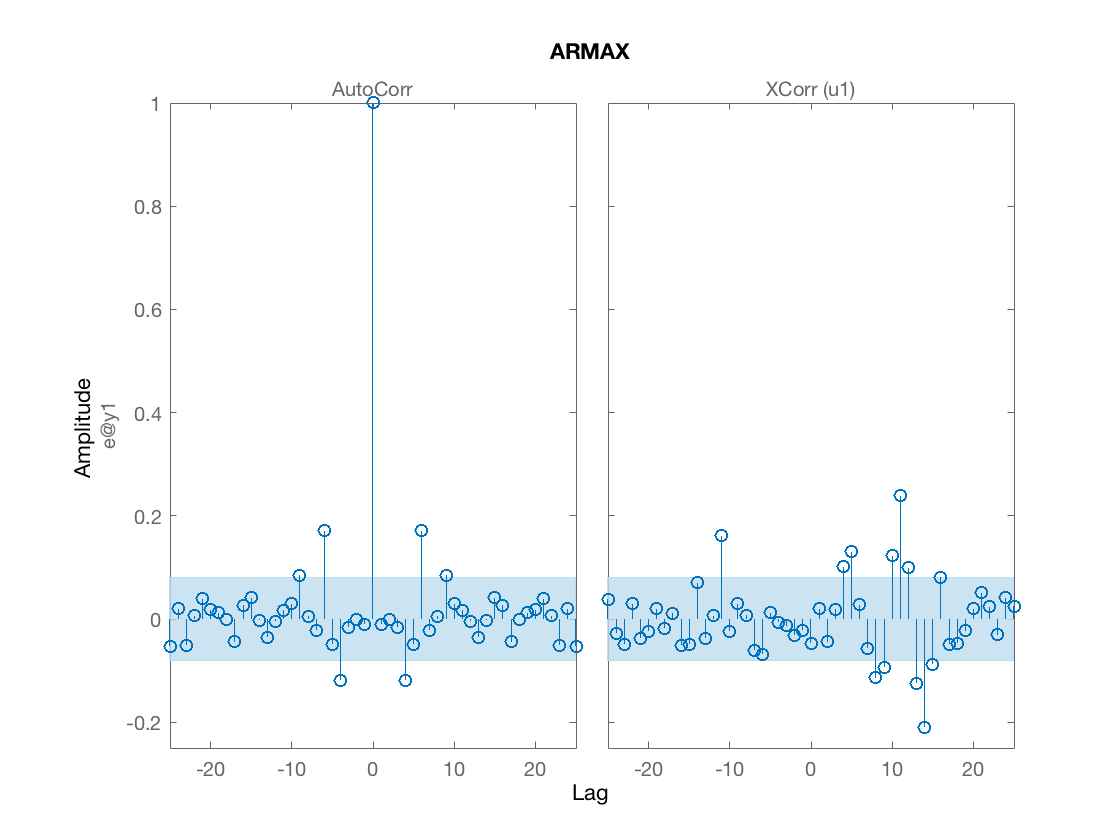
\includegraphics[height=5.5cm]{figures/v_armax.png}
		\subcaption{Whiteness test and cross-correlation test of the ARMAX model}\label{fig:v_armax}
	\end{subfigure}\hfill
	\begin{subfigure}{.49\textwidth}
		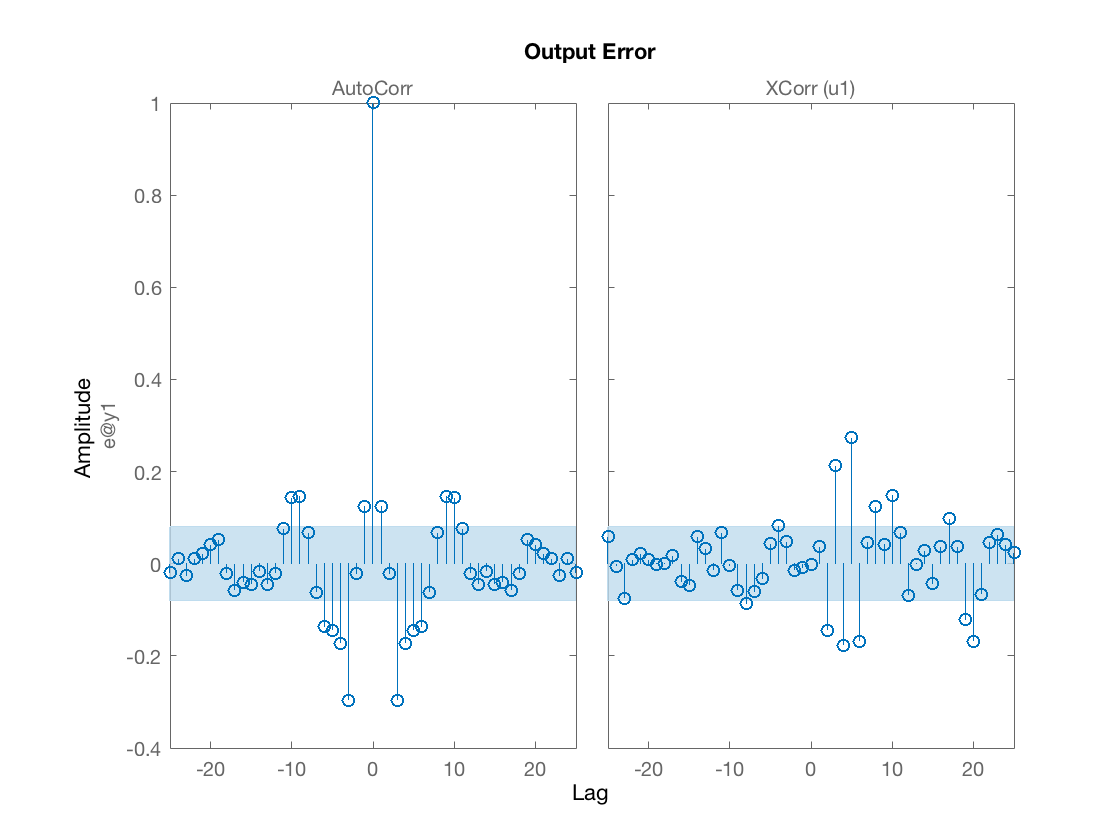
\includegraphics[height=5.5cm]{figures/v_oe.png}
		\subcaption{Whiteness test and cross-correlation test of the Output Error model}\label{fig:v_oe}
	\end{subfigure}
	\begin{subfigure}{.49\textwidth}
		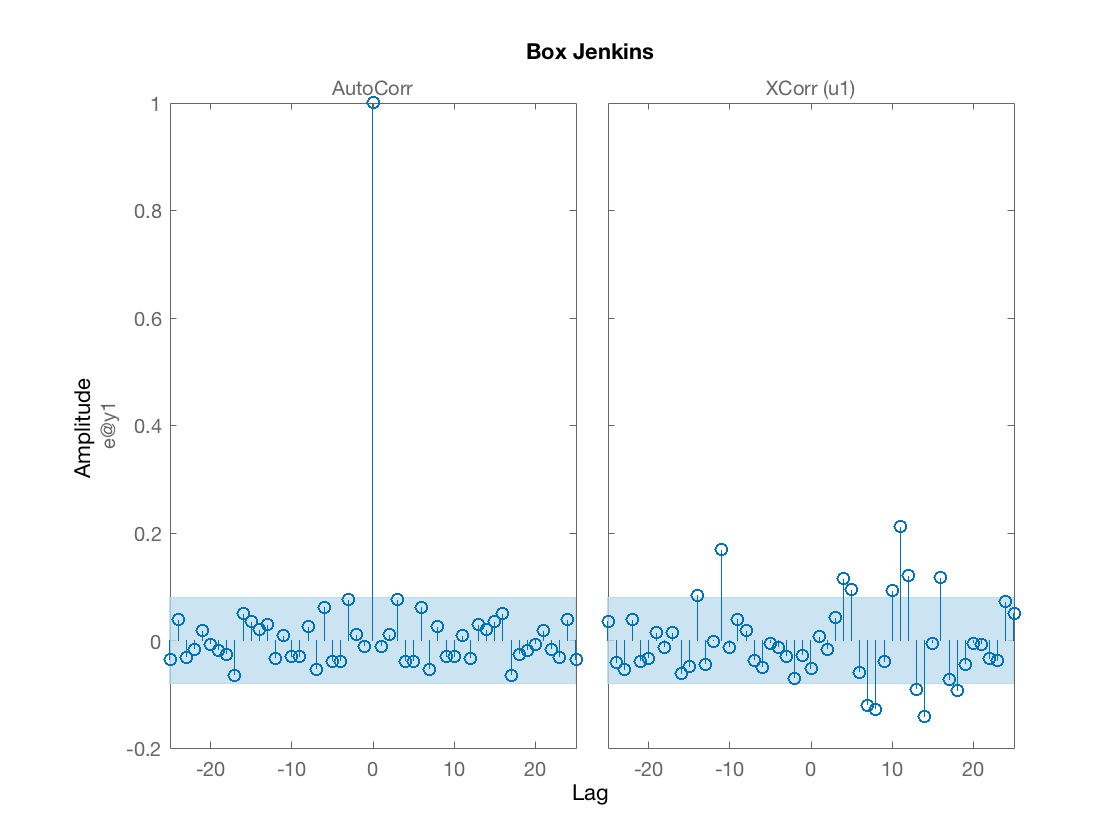
\includegraphics[height=5.5cm]{figures/v_bj.png}
		\subcaption{Whiteness test and cross-correlation test of the Box Jenkins model}\label{fig:v_bj}
	\end{subfigure}\hfill
	\begin{subfigure}{.49\textwidth}
		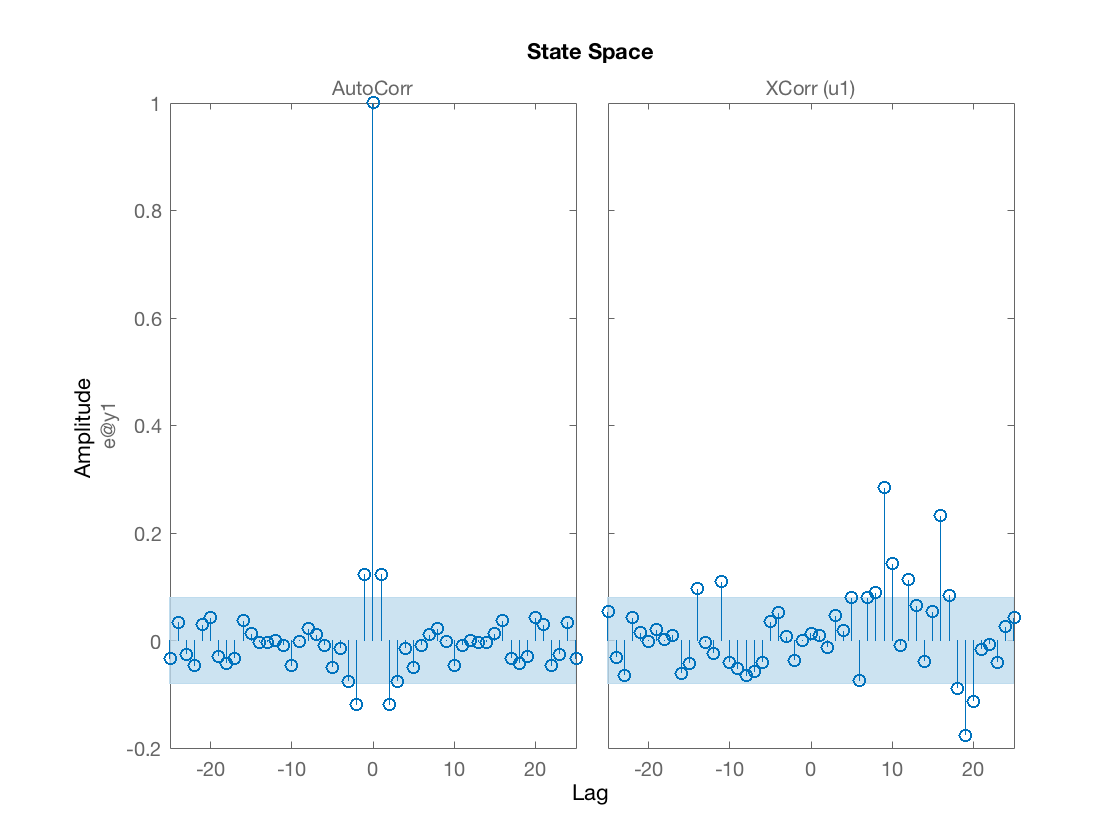
\includegraphics[height=5.5cm]{figures/v_ss.png}
		\subcaption{Whiteness test and cross-correlation test of the State Space model}\label{fig:v_n4sid}
	\end{subfigure}
	\caption{Whiteness test of the residuals and cross-correlation of the residuals and past inputs of different models with the MATLAB command \texttt{resid}.}
	\label{fig:test}
\end{figure}

